\section{Existing technologies}
This section will contain an analysis of existing technologies used for golf course maintenance. The aspects covered are according to the interview answers.

\subsection{Rain Bird SMRT-Y}
Rain Bird created the sensor SMRT-Y that measures soil moisture and displays it on a simple user interface\cite{smrty}].
The system from Rain Bird requires the use of Rain Bird irrigation, as the system is directly connected to the irrigation system. 
According to Rain Bird, this system provides over 40\% in water savings\cite{smrty2}.

SMRT-Y is fully automatic and requires no maintenance. Once buried it decides if the irrigation system should be turned on, based on the soil moisture. 
The only setup required is to set the threshold of the area where the sensor and irrigation system is located\cite{smrty2}.

The sensors are small and therefore well suited to bury around the course. But is required to be in close proximity of irrigation valves, which might not be useful everywhere.
The system does not send data to a central unit, making it hard to use to determine the soil moisture, but instead makes decisions for the greenkeepers. 

\subsection{Toro Turf Guard\texttrademark{}}
The company Toro created the Turf Guard\texttrademark{} sensors that allows greenkeepers to keep track of sensor data in real time. The sensors measure moisture, temperature, and salinity in the soil\cite{turfGuard}.
The sensors are wireless and has a range of 152 meters, but can be connected to repeaters to get a range of 1500 meters\cite{turfGuard}. It runs on the 900MHz ISM band, which requires no registration.

\begin{wrapfigure}{r}{0.4\textwidth}
\begin{center}
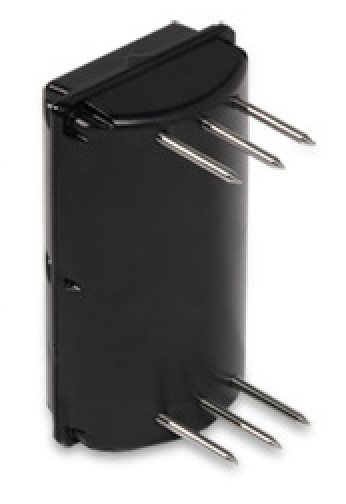
\includegraphics[width=0.3\textwidth]{chapters/analysis/figs/Turfguard.png}
\caption{Toro Turf Guard\texttrademark{} sensor\cite{turfGuard2}.}
\label{fig:turfguard}
\end{center}
\end{wrapfigure}

Turf Guard\texttrademark{} sensors are designed with two layers of sensors, allowing them to measure in the top soil and further down with one device.

The size of device allows it to fit into a standard hole-size, making them well suited to install on greens where a tool for creating holes are used\cite{turfGuard2}.

The entire system can be monitored from a computer, where the data are transmitted and shown in a user interface with locations for sensors available\cite{turfGuard2}.

The system requires the usage of other Toro systems to be working, making it hard to implement if systems from another manufacturer is already used. It also requires the use of repeaters close to the sensors, for transmitting data to the main device\cite{turfGuard2}.
